\section{Proof}
\label{sec:proof}

\section{Overlapping Freeze Windows}

The freeze windows for our algorithm are chosen specifically to ensure
that there is some point in time when all of the nodes are
frozen. Each node knows the intended freeze time. However, since their
clocks aren’t perfect, they don’t know exactly when it is.

Recall that our algorithm calls for each node to start its freeze
window when its clock reads $T - U_i$, and completes it when its clock
reads $T + U_i$, where $T$ is the freeze time and $U_i$ is NTP’s uncertainty
at that time. Since NTP guarantees that the real time $T$ will be within
the uncertainty bounds of when the node’s clock reads $T$, we can be
sure that each node will be frozen at the freeze time. Therefore, we
can be certain that their freeze windows overlap. The figure below
demonstrates four freeze windows at the freeze time of 8pm.

\begin{figure}[h]
  \centering
  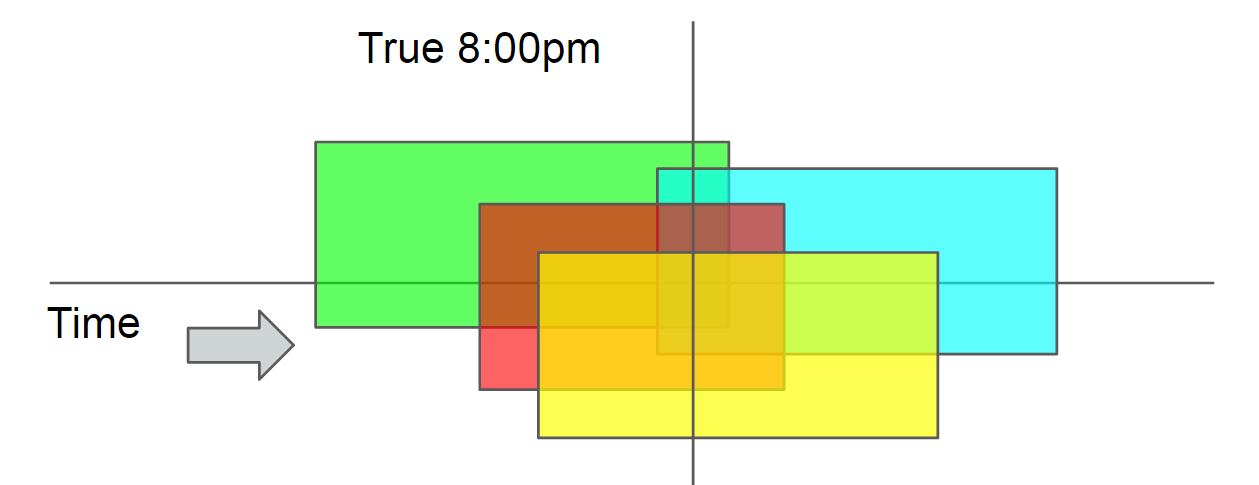
\includegraphics[width=0.8\textwidth]{overlapping-windows.png}
\end{figure}

\section{Consistency}

Our algorithm is designed to take consistent snapshots. A snapshot
would be inconsistent if it captured an event, but not an earlier
event that caused it. Let A be some event that caused B, another
event. For example, A could be a new class that we’re adding to a
library and B could be unit tests for that class. If we captured B in
our snapshot, but not A, our snapshot would contain the unit tests for
a class that doesn’t exist. This would cause the test suite to fail or
crash, which could be very bad. Therefore, it’s important that, if our
snapshot captures an event, that it also captures all events that
caused it as well. Formally, here is the statement that we want to
prove:

Let $A$ and $B$ be events in our system, where $B$ was caused by
$A$. If $B$ was captured in our snapshot, then $A$ must have been as
well.

Firstly, let’s define $T_A$ to be the time at which $A$ occurred and
$T_B$ to be the time at which B occurred. Since A caused B, we know
that A must have taken place before B, meaning $T_A< T_B$.

Our solution guarantees that all of the freeze windows of the nodes in
our system will overlap at some point in time, meaning that, for some
point in time, all nodes will be frozen. Now, it’s likely that the
freeze windows will all overlap for some interval, not for only a
single moment in time. During this interval, the cluster will not
respond to write events. Therefore, when we are considering the order
of events, we can collapse that whole interval into a single event and
we can consider the start time of the interval to be the time of the
event. Let’s call the event $F$ and its time $T_F$.

Let’s assume, for the sake of contradiction, that there is a series of
events that could violate our proposed invariant. More specifically,
let’s assume that it is possible for B to have been captured in the
snapshot while A was not.

Each node’s portion of the snapshot is taken when that node
freezes. No other events will occur on the node between when it takes
its snapshot (i.e. the beginning of its freeze interval) and $F$, the
moment when all nodes are frozen. Therefore, if $B$ was included in
the snapshot, it must have happened before $F$, meaning $T_B <
T_F$. Since $A$ was not captured in the snapshot, it must have
happened after $F$, meaning that $T_F<T_A$. We can combine these two
inequalities together to get $T_B< T_A$.

This contradicts the original requirement that A must have taken place
before $B$, or $T_A< T_B$. Therefore, since we have reached a
contradiction, we know that our original assumption must have been
incorrect and, therefore, our statement must be true.

Since our statement is true for any two events in our system with a
causal relationship, we know that our snapshot must be consistent.

\section{Performance}

There are a number of different performance characteristics that need
to be considered to ensure that our algorithm will not have an adverse
impact on the current functionality of Ceph. First, we need to
consider the impact of delaying writes for a freeze. Since each node
freezes for the uncertainty that is determined by the time protocol,
the magnitude of the uncertainty is dependent on which time
synchronization protocol is used. We analyze the uncertainty that NTP
provides later in this document and discuss what impact our solution
would have on a Ceph instance if NTP is used as the time
synchronization protocol. However, if a time synchronization protocol
could provide uncertainties in 10-20 millisecond range, giving 20-40
millisecond freeze windows, our algorithm shouldn’t impact the
cluster’s performance significantly. Also, freeze windows of each of
the nodes is offset from each other, which means that the whole Ceph
instance is frozen for a much shorter period of time.

Next, we consider the networking requirements of this algorithm. We
need to be assured that our algorithm does not require significant
amounts of bandwidth which would cause network congestion within a
Ceph instance. Since most Ceph instances are already running a time
synchronization protocol like NTP, our algorithm does not require any
extra messages during the sync/update phase. The freeze phase also
does not require any extra messages. The number of success/failure
messages required in the confirmation phase is $O(n)$ in the size of
the instance and thus would not have a significant impact on the
performance of the instance (because each message would be only a few
bytes). In the replication phase, the remote instance needs to read
the data from the local one, but this cost is inherent to any
snapshotting algorithm and thus not a negative characteristic of ours
in particular.

Finally, we need to consider whether this algorithm will place a
significant computational burden on nodes. Each primary OSD needs to
send its PGs' information to the remote instance. This should not
impact the performance of the primaries, since it shouldn’t take too
long to send all of that information. Even if it did take a while to
send the information, read and write requests could still be addressed
by prioritizing those requests above the requests for the objects from
the remote instance. Sending all of the information out at once could
use a lot of bandwidth, but since it is distributed throughout the
Ceph instance, the choke point would be the bandwidth from the local
instance to the remote instance, which should be pretty large and not
a concern if we prioritize normal client traffic over the
inter-instance traffic.

If the user wants to store the uncertainty information of the nodes in
the monitors, the monitor nodes will have to store the uncertainty of
each node in the local instance. Though there could be tens of
thousands of OSDs, storing even eight bytes of time information would
only be a couple of kilobytes of data. Even if it took a megabyte to
store all of the timestamps, it would not be a significant memory
burden. Also, reporting clock information to the monitors would
require a constant number of messages for each node and, therefore,
only a linear number of messages in the number of nodes in the
instance.  Based on our analysis, our algorithm should not have a
significant impact on the performance of the Ceph instance.
